\documentclass{article}
\usepackage{graphicx} % Load the graphicx package
\usepackage{amsmath} % Required for math symbols like \frac


\begin{document}
\title{Exercício 9} 
\author{Arthur Felipe Reis Souza}
\date{\today}
\maketitle


\section{Introduction}

\vspace{10pt}

As redes neurais MLP (Multi Layer Perceptron) são úteis em problemas de regressão, classificação e previsão. Portanto, pode ser considerada como uma rede neural aproximadora universal de funções. O exercício consiste em utilizar uma rede neural MLP, com 1 camada intermediária contendo 3 neurônios, para aproximar uma função senoidal durante um período.

\section{Desenvolvimento}

\vspace{10pt}

A função senoidal foi gerada e somada a um ruído gaussiano, após isso os dados de treinamento e teste foram gerados.

\vspace{10pt}

\begin{figure}[h]

    \centering
    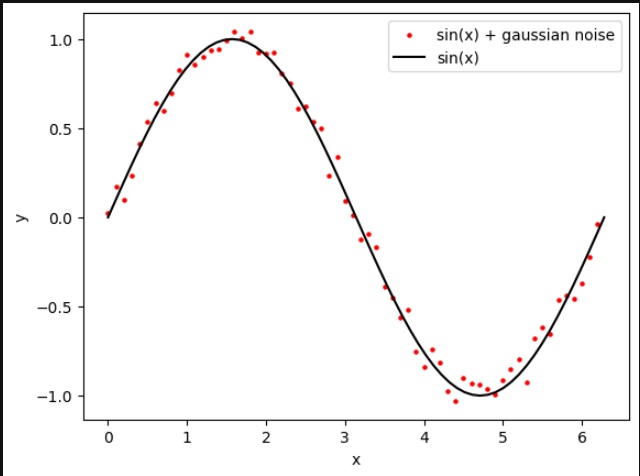
\includegraphics[height=2.5in]{func_sin_noise.png}
    \caption{Função senoidal com ruído gaussiano.}
    \label{fig:example}
    
\end{figure}

\vspace{10pt}

Após o treinamento da rede, foram utilizados dados de teste variando no intervalo de \(0\) a \(2\pi\). 6 aproximações foram realizadas, em cada aproximação foi variado um ou mais hyperparâmetros. A métrica utilizada para avaliar o modelo foi o erro médio quadrático (MSE).

\vspace{10pt}

\section{Resultados}

\vspace{10pt}

Os resultados obtidos para cada aproximação estão registrados abaixo : 


\vspace{10pt}

\begin{figure}[h]

    \centering
    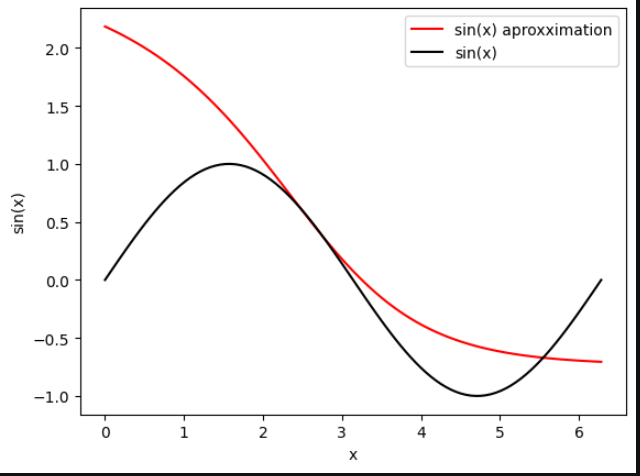
\includegraphics[height=1in]{sin_ap1.png}
    \caption{Função senoidal com $\eta$ 0.1 and max epochs : 100.}
    \label{fig:example}
    
\end{figure}

\vspace{10pt}




\vspace{10pt}

\begin{figure}[h]

    \centering
    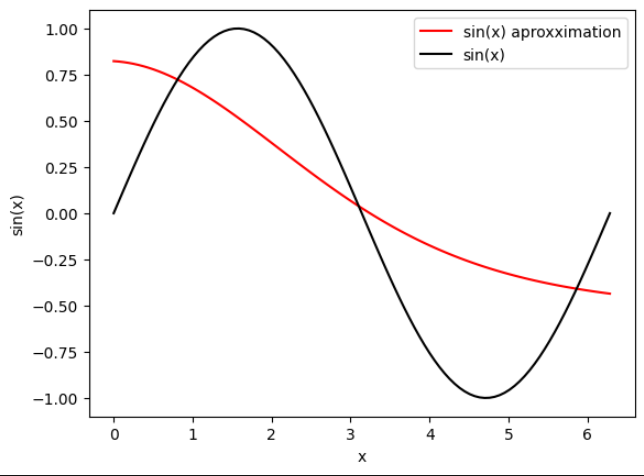
\includegraphics[height=1in]{sin_ap2.png}
    \caption{Função senoidal com $\eta$ 0.01 and max epochs : 100.}
    \label{fig:example}
    
\end{figure}

\vspace{10pt}


\vspace{10pt}

\begin{figure}[h]

    \centering
    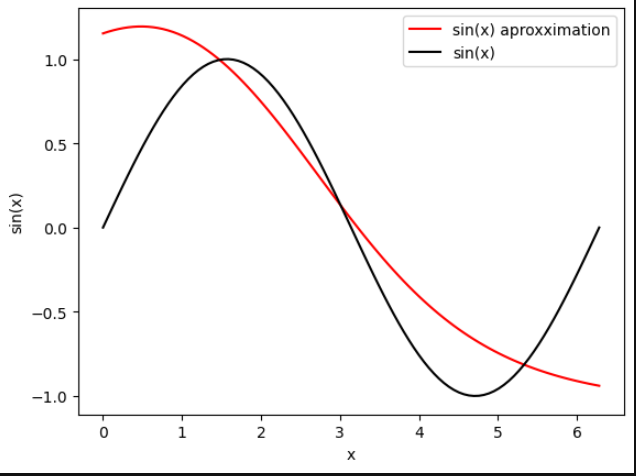
\includegraphics[height=1in]{sin_ap3.png}
    \caption{Função senoidal com $\eta$ 0.01 and max epochs : 500.}
    \label{fig:example}
    
\end{figure}

\vspace{10pt}


\vspace{10pt}

\begin{figure}[h]

    \centering
    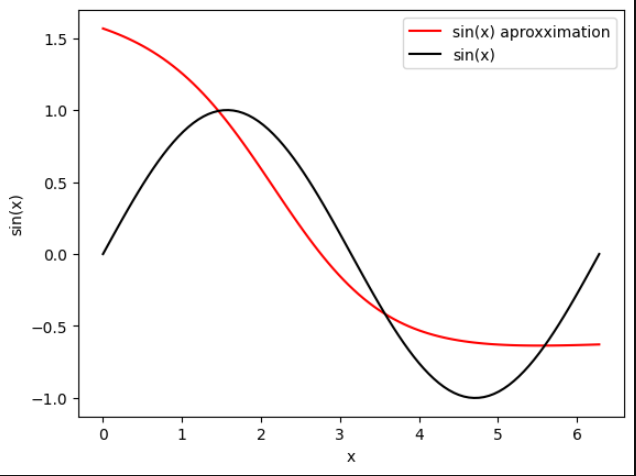
\includegraphics[height=1in]{sin_ap4.png}
    \caption{Função senoidal com $\eta$ 0.01 and max epochs : 1000.}
    \label{fig:example}
    
\end{figure}

\vspace{10pt}

\vspace{10pt}

\begin{figure}[h]

    \centering
    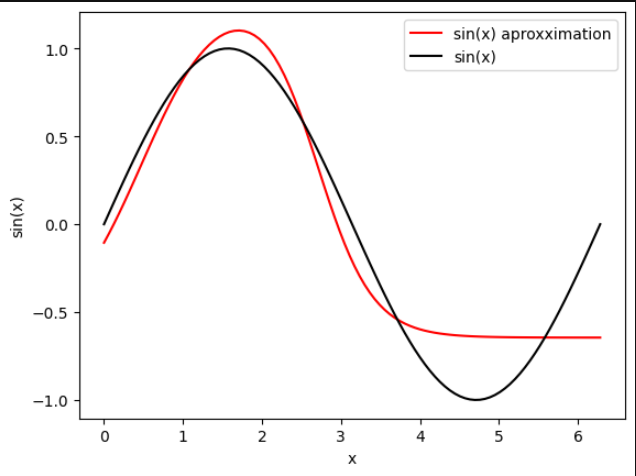
\includegraphics[height=1in]{sin_ap5.png}
    \caption{Função senoidal com $\eta$ 0.1 and max epochs : 1000.}
    \label{fig:example}
    
\end{figure}

\vspace{10pt}

\vspace{10pt}

\begin{figure}[h]

    \centering
    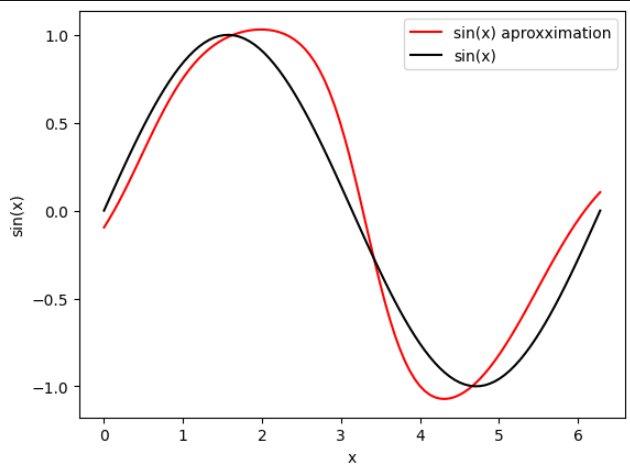
\includegraphics[height=1in]{sinc_ap6.png}
    \caption{Função senoidal com $\eta$ 0.1 and max epochs : 10000.}
    \label{fig:example}
    
\end{figure}

\vspace{10pt}

Pode se observar, analisando as figuras acima que ao aumentar o número de épocas a aproximação aparenta ser melhor. A variação do learning rate também influência na aproximação do modelo, sendo nesse exemplo $\eta$ = 0.1 resultando nas melhores aproximações. A figura abaixo é uma tabela contendo os resultados para os 6 modelos construídos.

\vspace{10pt}

\begin{figure}[h]

    \centering
    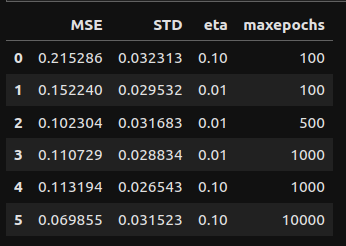
\includegraphics[height=1.25in]{table_result.png}
    \caption{Tabela contendo os resultados para cada variação de hyperparâmetro.}
    \label{fig:example}
    
\end{figure}

\vspace{10pt}

\newpage

\section{Conclusão}

\vspace{10pt}

Portanto, ao realizar o exercício com êxito é possível observar uma rede neural MLP aproximando uma função senoidal. Ao variar os hyperparâmetros da rede, resultados diferentes foram obtidos, sendo que o melhor resultado foi utilizando $\eta$ = 0.1 e um número máximo de epocas de 10000. Há várias variações das redes MLP, com diferentes tipos de otimizadores e diferentes tipos de $\eta$ que também pode ser adaptativo. Cabe a quem estar construindo o modelo realizar uma análise profunda dos dados e escolher o modelo que tem uma melhor performance de acordo com uma métrica de escolhida.




\end{document}